\section{Outil de gestion de l'inventaire proposé}\label{sec:meth_tool}
La section \ref{sec:meth_urb_based_inventory} a décrit la méthode utilisée pour entreposer les informations réglementaires et calculer un inventaire à partir de ces informations. Cependant, la création de cette réglementation est onéreuse et peu intuitive. Cette section visera à proposer un outil qui permet de générer la réglementation, d'en extraire l'information pertinente, et de permettre à des praticiens d'accéder à l'inventaire pour d'autres études. La section est divisée comme suit:
\begin{itemize}
    \item Définition des requis
    \item Architecture de l'outil logiciel
    \item Survol des fonctions de l'API
    \item Survol de l'interface web établi
\end{itemize}
\subsection{Requis}
\paragraph{Interface avec la base de données et cohérence des données}
En premier lieu, il doit être possible de créer, modifier et supprimer des données sur la base de données tout en assurant la cohérence des données. Ainsi, les fonctions de suppression et de modification doivent assurer que les données restent valides pour permettre le calcul de l'inventaire à la demande de l'utilisateur. Idéalement, il serait possible d'automatiser des fonctionnalités de validation de la base de données pour trouver de potentielles erreurs dans les données fournies.
\paragraph{Calcul réglementaire basé sur les données foncières}
L'interface doit permettre la création d'un inventaire à partir des données du rôle foncier au moyen  de l'algorithme détaillé dans la section \ref{sec:meth_urb_based_inventory}. Il devrait ensuite être possible de valider l'inventaire contre les données présentement sauvegardées dans la base de données si des entrées existent déjà pour les lots.
\paragraph{Calcul réglementaire avec entrée manuelle}
Environ 50\% des entrées commerciales dans le rôle foncier n'ont pas de superficie listée. Sachant qu'une importante partie des règlements est dépendante de la superficie de plancher pour déterminer la capacité, il est important de faire une entrée semi-manuelle où l'utilisateur peut entrer la superficie ou tout autre paramètre et permettre de faire le calcul à partir de ces entrées manuelles.  
\paragraph{Entrée manuelle d'un inventaire}
L'outil doit permettre d'entrer un inventaire manuellement si l'utilisateur veut entrer manuellement une valeur mesurée sur le terrain.
\paragraph{Comparaison des ensembles de règlements} L'outil doit permettre de faire une comparaison graphique entre différents ensembles de règlements pour différentes utilisations du sol en fonction du temps et de la géographie.
\paragraph{Visualisation de l'inventaire sur un territoire} L'outil devra permettre une représentation graphique de l'inventaire à différents niveaux d'agrégation (quartier, territoire complet).
\paragraph{Accessibilité à partir de tierces parties} Une partie ou l'ensemble des données devra être accessible à partir d'autres scripts au moyen d'une API. Le but sera ici d'assurer que les données générées puissent être utilisées pour comprendre l'effet de l'offre de stationnement sur les comportements de mobilité dans le contexte québécois.
\subsection{Architecture de l'outil proposé}
Différentes solutions peuvent être envisagées pour gérer des données spécialisées. Un inventaire de stationnement pourrait être généré et interprété dans différents logiciels (SIG, tableurs) mais cela rend la création, le maintien et l'interprétation de l'inventaire complexes. Alternativement, un outil spécialisé peut être généré. Ce dernier peut être une application sur les ordinateurs personnels de différents analystes ou une application web avec une infrastructure centralisée pour faire les calculs et publier l'information, ou une solution hybride avec une infrastructure centralisée qui est utilisée pour la sauvegarde des données avec un outil local pour manipuler les valeurs. \par
La solution entièrement en ligne a été retenue pour plusieurs raisons. Premièrement, cela évite la duplication d'information et permettrait à un organisme de maintenir l'inventaire et de le rendre disponible à d'autres analystes pour faire des analyses de mobilité. D'autre part, cela permet de centraliser les ressources de calcul et de permettre de mettre à jour l'outil au besoin. Ce type d'implémentation serait aussi compatible avec l'utilisation des données par d'autres applications au besoin au moyen de l'\ac{API}. Le diagramme \ref{fig:architecture_outil} montre comment les différents utilisateurs et grands blocs interagissent.\par
\begin{figure}[h]
    \centering
    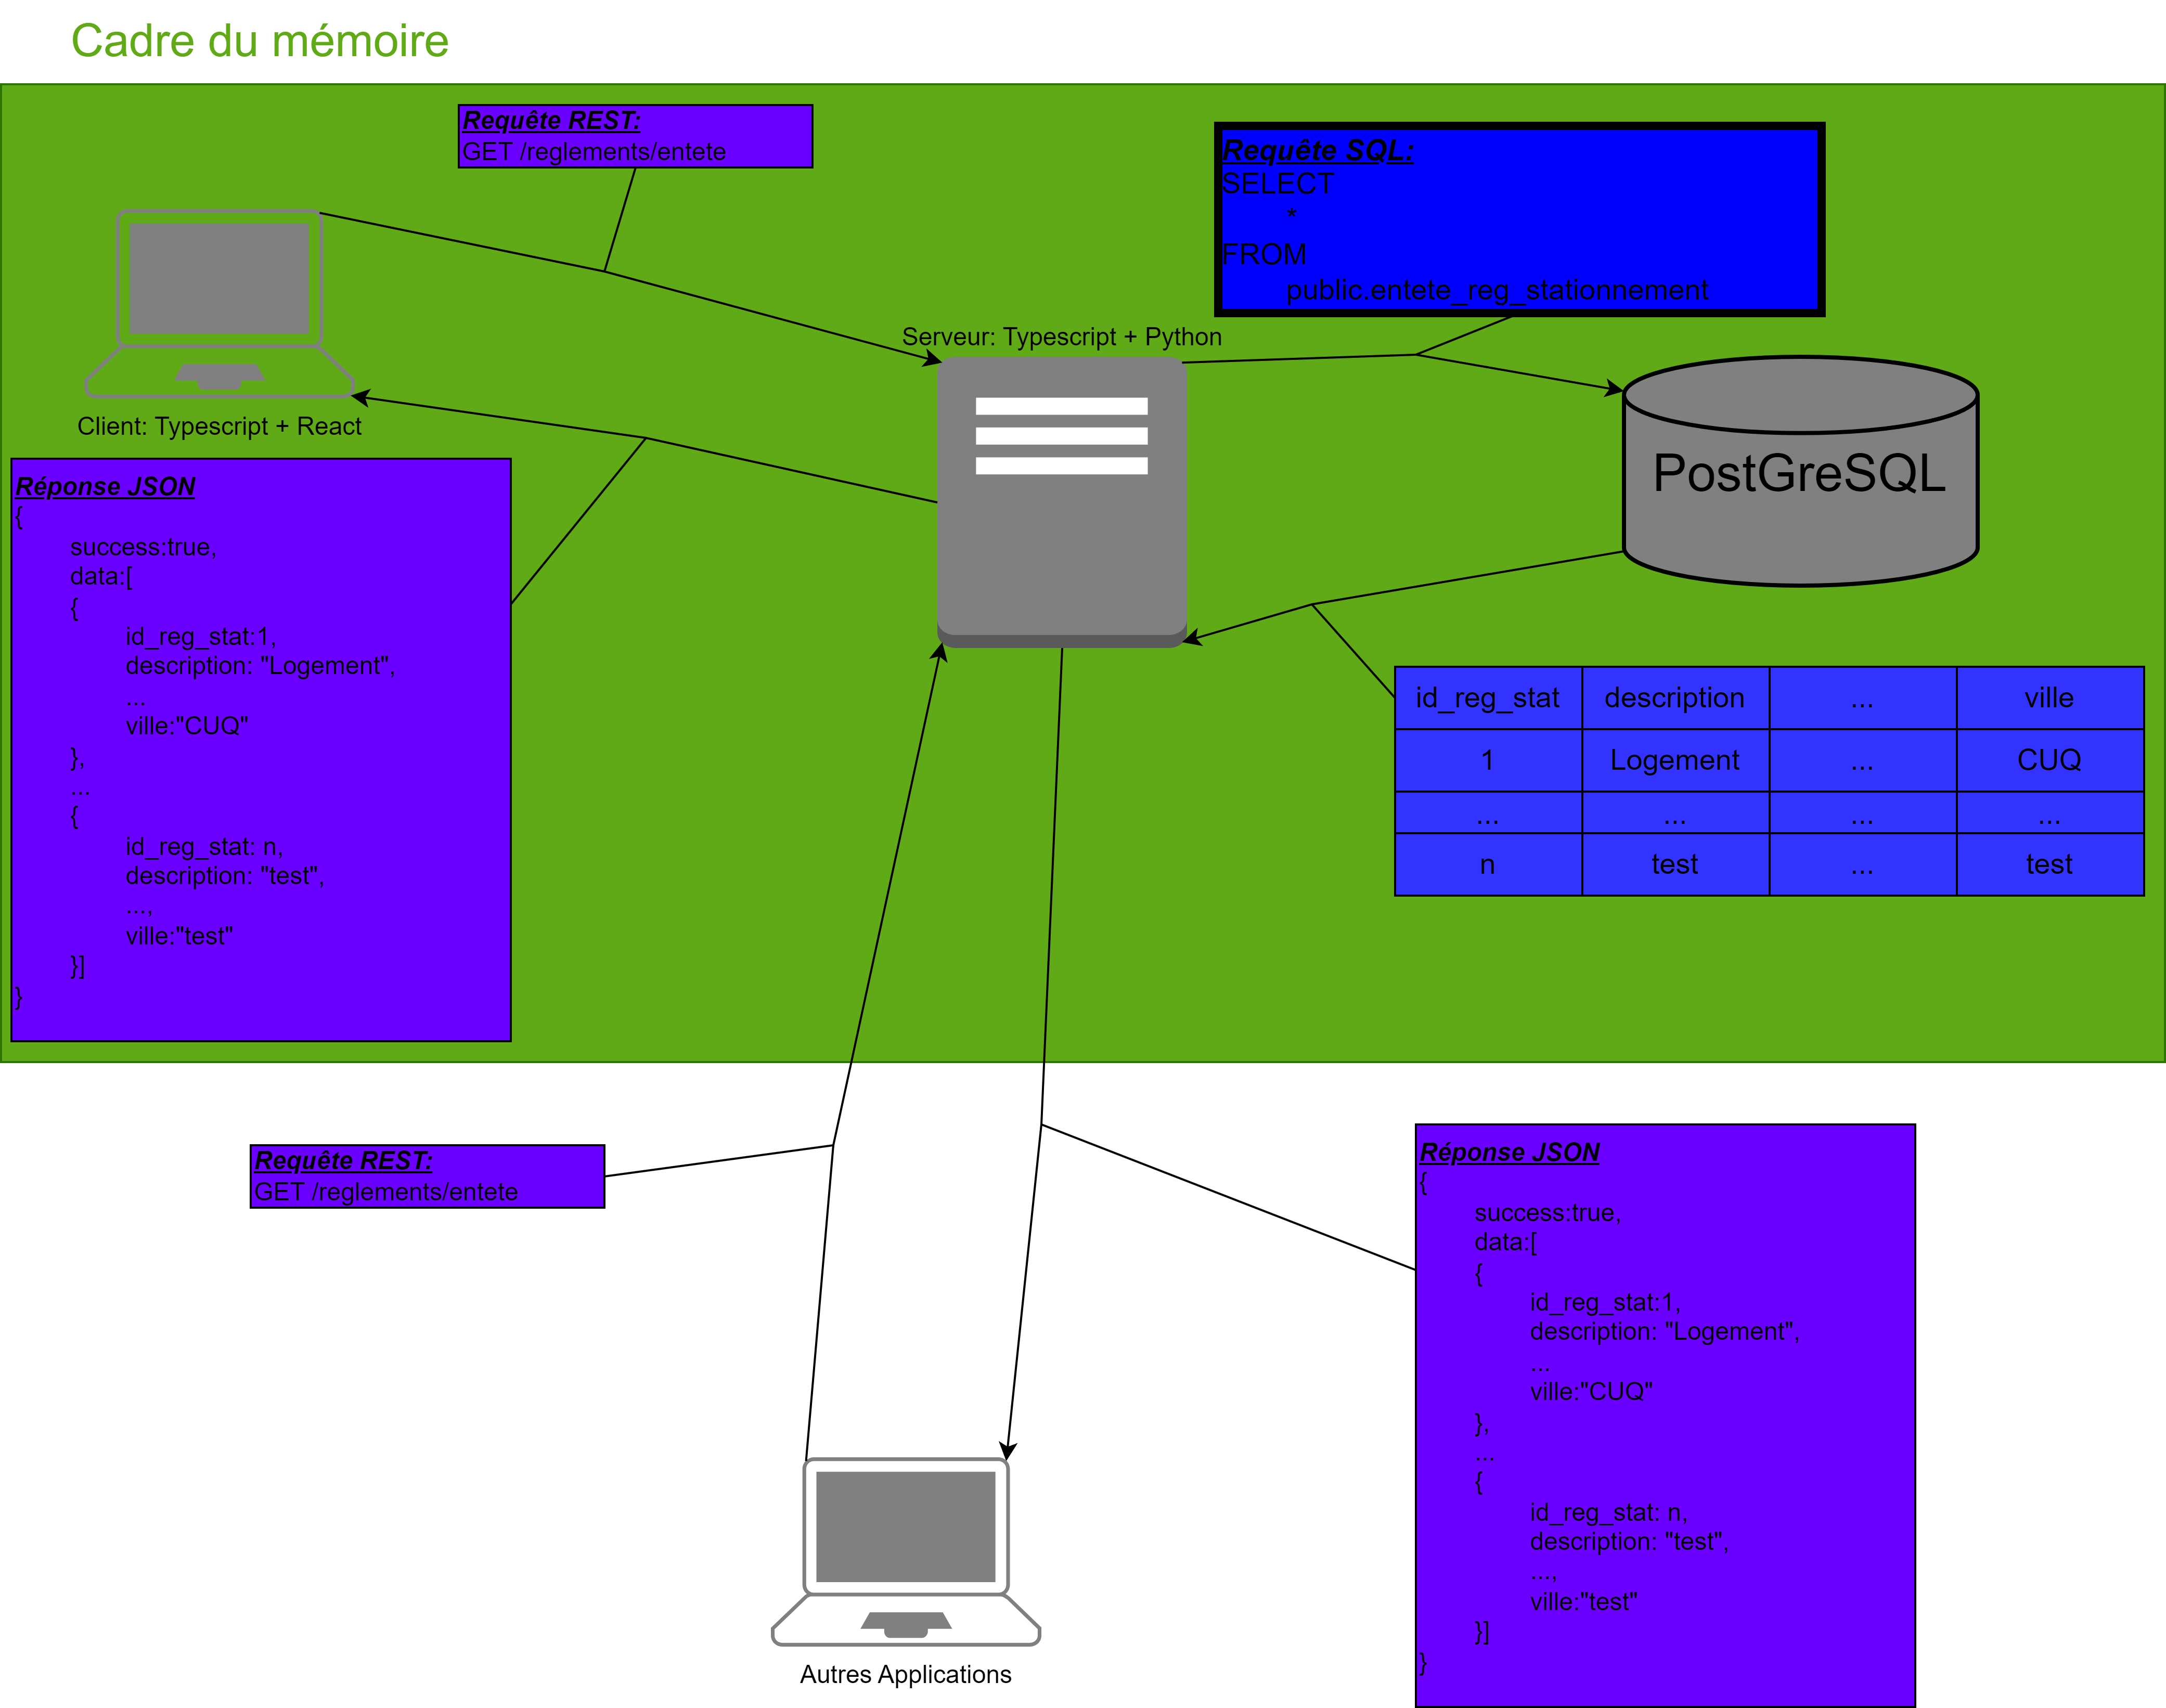
\includegraphics[width=1.0\linewidth]{dia/Architecture_outil.png}
    \caption{Architecture de l'outil développé dans le cadre du mémoire}
    \label{fig:architecture_outil}
\end{figure}
Ce type d'arrangement est typique dans les applications web \cite{chernenko_full_2024}. Dans ce cas, un morceau de code TypeScript est téléchargé sur la machine \og{client} \fg{} qui fait le rendu de l'application. Les informations et les données sont demandées par la machine \og{client} \fg{} au travers de l'API qui renvoie les données pertinentes à la requête. 
